\documentclass[aspectratio=169,12pt,t]{beamer}

% --- Theme: Metropolis (modern, clean) ---
\usetheme[progressbar=frametitle,numbering=fraction,block=fill]{metropolis}

% --- Fira Sans font (install texlive-fonts-extra if missing) ---
\IfFileExists{FiraSans.sty}{\usepackage[sfdefault]{FiraSans}}{}

% --- Light background with warm accent ---
\definecolor{mDarkTeal}{RGB}{35,55,59}
\definecolor{mLightBrown}{RGB}{235,228,216}
\definecolor{mAccent}{RGB}{140,70,20}

\setbeamercolor{normal text}{fg=mDarkTeal,bg=white}
\setbeamercolor{alerted text}{fg=mAccent}
\setbeamercolor{frametitle}{bg=mDarkTeal,fg=white}
\setbeamercolor{progress bar}{fg=mAccent,bg=mLightBrown}
\setbeamercolor{title separator}{fg=mAccent}
\setbeamercolor{progress bar in head/foot}{fg=mAccent,bg=mLightBrown}
\setbeamercolor{progress bar in section page}{fg=mAccent,bg=mLightBrown}

% --- Packages ---
\usepackage[utf8]{inputenc}
\usepackage{amsmath,amssymb,amsthm}
\usepackage{mathrsfs}
\usepackage{tikz}
\usetikzlibrary{arrows.meta,positioning,calc,decorations.pathreplacing,shapes,patterns}
\usepackage{pgfplots}
\pgfplotsset{compat=1.18}

% --- Semi-transparent white highlight for text on top of background images ---
\usepackage[most]{tcolorbox}

% Inline highlight: \hl{short text}
\newtcbox{\hl}{%
  nobeforeafter, tcbox raise base,
  colback=white, opacityback=0.6,
  colframe=white, opacityframe=0,
  sharp corners, boxsep=2pt, left=3pt, right=3pt, top=2pt, bottom=2pt%
}

% Block highlight: \begin{hlbox} ... \end{hlbox}  (multi-line, paragraphs, itemize)
% Optional argument accepts any tcolorbox key, e.g. [width=0.6\linewidth]
\newtcolorbox{hlbox}[1][]{%
  enhanced, breakable,
  colback=white, opacityback=0.6,
  colframe=white, opacityframe=0,
  boxsep=3pt, left=6pt, right=6pt, top=4pt, bottom=4pt,
  sharp corners,
  {#1}%
}

% --- Custom colors for content types ---
\definecolor{defcolor}{RGB}{25,85,120}
\definecolor{thmcolor}{RGB}{140,35,35}
\definecolor{proofcolor}{RGB}{35,100,50}
\definecolor{excolor}{RGB}{140,75,10}
\definecolor{remcolor}{RGB}{90,90,90}

% --- Beamer blocks for mathematical content types (semi-transparent) ---
% Native Beamer blocks cannot carry an alpha channel, so we render the blocks
% with tcolorbox instead. Title and body are both at 50% opacity; body tint
% bumped from !5 to !15 to stay visible after the alpha is applied.
\tcbset{hlblockbase/.style={
  enhanced, breakable,
  coltitle=white, fonttitle=\bfseries,
  opacitybacktitle=0.8, opacityback=0.6,
  opacityframe=0,
  sharp corners,
  boxsep=1pt, left=5pt, right=5pt, top=2pt, bottom=2pt,
  toptitle=1pt, bottomtitle=1pt
}}

\newtcolorbox{defblock}[1]{hlblockbase, title={#1},
  colbacktitle=defcolor, colback=defcolor!15, colframe=defcolor}
\newtcolorbox{thmblock}[1]{hlblockbase, title={#1},
  colbacktitle=thmcolor, colback=thmcolor!15, colframe=thmcolor}
\newtcolorbox{proofblock}[1]{hlblockbase, title={#1},
  colbacktitle=proofcolor, colback=proofcolor!15, colframe=proofcolor}
\newtcolorbox{exblock}[1]{hlblockbase, title={#1},
  colbacktitle=excolor, colback=excolor!15, colframe=excolor}
\newtcolorbox{remblock}[1]{hlblockbase, title={#1},
  colbacktitle=remcolor, colback=remcolor!15, colframe=remcolor}

% --- Metadata ---
\title{Chapter 2: Basic Topology}
\subtitle{Section: Metric Spaces}
\author{Based on Walter Rudin's \emph{Principles of Mathematical Analysis}}
\date{}

\begin{document}

{
\usebackgroundtemplate{%
  
\includegraphics[width=\paperwidth,height=\paperheight,keepaspectratio=false]{chapter_02_bg_00.png}%
}
% =============================================================================
\begin{frame}
  \titlepage
  \note{
    Welcome to Chapter 2 of Principles of Mathematical Analysis. In this
    section we study metric spaces, which provide the natural setting for
    discussing limits, continuity, and convergence. A metric space is simply
    a set equipped with a notion of distance. This abstraction lets us do
    analysis not just on the real line, but in much more general settings.
  }
\end{frame}
}

{
\usebackgroundtemplate{%
  
\includegraphics[width=\paperwidth,height=\paperheight,keepaspectratio=false]{chapter_02_bg_01.png}%
}
% =============================================================================
\begin{frame}[c]{Outline}
  \begin{center}
    \tableofcontents
  \end{center}
  \note{
    Here is an outline of what we will cover. We begin by defining metric
    spaces and looking at key examples. Then we introduce the fundamental
    topological concepts: neighborhoods, limit points, open sets, closed sets,
    and more. After that we prove the basic theorems about open and closed
    sets, including De Morgan's laws and closure properties under unions and
    intersections. Finally we discuss the closure of a set and the notion of
    relative topology.
  }
\end{frame}

% =============================================================================
\section{Metric Spaces: Definitions and Setup}

% =============================================================================
% --- 2.15 Definition: Metric Space ---
% =============================================================================

% --- Build 1/3 ---
\begin{frame}{Definition 2.15: Metric Space}
  \begin{defblock}{Definition 2.15}
    A set $X$ is a \alert{metric space} if with any two points $p, q \in X$ there is
    associated a real number $d(p, q)$, called the \alert{distance}, such that:
    \begin{enumerate}
      \item[(a)] $d(p, q) > 0$ if $p \neq q$;\quad $d(p, p) = 0$
    \end{enumerate}
  \end{defblock}

  \note{
    Let us define the central object of this section. A metric space is a set
    equipped with a distance function satisfying certain axioms. The first
    axiom, positivity, is what prevents the notion of distance from being
    trivial. Without it, two different points could have distance zero, and
    we would lose the ability to distinguish them metrically. Notice that
    the axiom has two parts: distinct points must have strictly positive
    distance, and the distance from any point to itself must be zero. This
    second part is a normalization. Next we see another fundamental property.
  }
\end{frame}

% --- Build 2/3 ---
\begin{frame}{Definition 2.15: Metric Space}
  \begin{defblock}{Definition 2.15}
    A set $X$ is a \alert{metric space} if with any two points $p, q \in X$ there is
    associated a real number $d(p, q)$, called the \alert{distance}, such that:
    \begin{enumerate}
      \item[(a)] $d(p, q) > 0$ if $p \neq q$;\quad $d(p, p) = 0$
      \item[(b)] $d(p, q) = d(q, p)$
    \end{enumerate}
  \end{defblock}

  \note{
    Symmetry says the distance from "p" to "q" is the same as from "q" to
    "p". This might seem obvious, but there are useful asymmetric notions
    of distance, such as travel time on one-way streets, that do not satisfy
    this axiom. By requiring symmetry, we ensure that distance behaves like
    our geometric intuition of length. The third property, the triangle
    inequality, is the most powerful of the three.
  }
\end{frame}

% --- Build 3/3 ---
\begin{frame}{Definition 2.15: Metric Space}
  \begin{defblock}{Definition 2.15}
    A set $X$ is a \alert{metric space} if with any two points $p, q \in X$ there is
    associated a real number $d(p, q)$, called the \alert{distance}, such that:
    \begin{enumerate}
      \item[(a)] $d(p, q) > 0$ if $p \neq q$;\quad $d(p, p) = 0$
      \item[(b)] $d(p, q) = d(q, p)$
      \item[(c)] $d(p, q) \leq d(p, r) + d(r, q)$, for any $r \in X$
    \end{enumerate}
  \end{defblock}

  \vspace{0.3em}
  \begin{hlbox}
    Any function with these three properties is called a \emph{distance function} or \emph{metric}.
  \end{hlbox}

  \note{
    The third property is the triangle inequality. It says that going from "p"
    to "q" directly is never longer than going from "p" to some intermediate
    point "r" and then from "r" to "q". This is the most substantial of the
    three axioms and plays a crucial role in many proofs. A function
    satisfying all three properties is called a distance function, or a metric.
  }
\end{frame}

% --- Diagram: Metric Space Axioms ---
\begin{frame}{Definition 2.15: Visualizing the Triangle Inequality}
  \begin{center}
  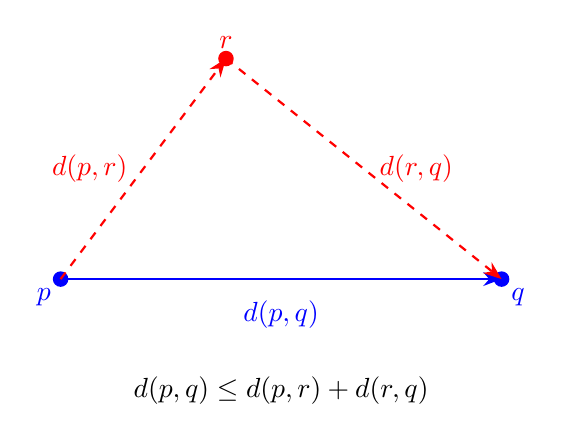
\begin{tikzpicture}[scale=1.4]
    \coordinate (p) at (0,0);
    \coordinate (q) at (4,0);
    \coordinate (r) at (1.5,2);

    \fill[blue] (p) circle (2pt) node[below left]{$p$};
    \fill[blue] (q) circle (2pt) node[below right]{$q$};
    \fill[red] (r) circle (2pt) node[above]{$r$};

    \draw[thick, blue, -{Stealth}] (p) -- (q)
      node[midway, below=4pt]{$d(p, q)$};
    \draw[thick, red, dashed, -{Stealth}] (p) -- (r)
      node[midway, left=2pt]{$d(p, r)$};
    \draw[thick, red, dashed, -{Stealth}] (r) -- (q)
      node[midway, right=2pt]{$d(r, q)$};

    \node[anchor=north] at (2,-0.8) {$d(p, q) \leq d(p, r) + d(r, q)$};
  \end{tikzpicture}
  \end{center}

  \note{
    As you can see, the direct path from "p" to "q" is never longer than the
    detour through "r". The triangle inequality is the workhorse of metric
    space theory. Almost every proof in this chapter uses it at some point.
    It is what makes neighborhoods well-behaved and allows us to control
    distances indirectly. Interestingly, equality holds in Euclidean space
    precisely when "r" lies on the line segment between "p" and "q".
  }
\end{frame}

% =============================================================================
% --- 2.16 Examples ---
% =============================================================================

% --- Build 1/2 ---
\begin{frame}{Examples 2.16: Euclidean Spaces}
  \begin{exblock}{Example 2.16: Euclidean Spaces}
    The most important metric spaces are the \alert{Euclidean spaces} $R^k$:
    \[
      d(\mathbf{x}, \mathbf{y}) = |\mathbf{x} - \mathbf{y}| \qquad (\mathbf{x}, \mathbf{y} \in R^k)
    \]
    Special cases: $R^1$ (the real line), $R^2$ (the complex plane).
  \end{exblock}

  \hl{By Theorem 1.37, this satisfies Definition 2.15.}

  \note{
    Euclidean spaces are by far the most important examples, and they are the
    setting for most of classical analysis. Verifying the triangle inequality
    for Euclidean distance is actually the hard part; that is what Theorem
    1.37 from Chapter 1 established using the Schwarz inequality. It is
    worth noting that the Euclidean metric is not the only way to measure
    distance in "R" to the "k". For instance, the maximum of the coordinate
    differences also defines a valid metric, but we will mostly work with
    the standard Euclidean one. Now let us see an important observation
    about subsets.
  }
\end{frame}

% --- Build 2/2 ---
\begin{frame}{Examples 2.16: Euclidean Spaces}
  \begin{exblock}{Example 2.16: Euclidean Spaces}
    The most important metric spaces are the \alert{Euclidean spaces} $R^k$:
    \[
      d(\mathbf{x}, \mathbf{y}) = |\mathbf{x} - \mathbf{y}| \qquad (\mathbf{x}, \mathbf{y} \in R^k)
    \]
    Special cases: $R^1$ (the real line), $R^2$ (the complex plane).
  \end{exblock}

  \begin{hlbox}
    By Theorem 1.37, this satisfies Definition 2.15.

    \vspace{0.5em}
    \textbf{Key observation:} Every subset $Y$ of a metric space $X$ is itself a metric space (with the same distance function).
  \end{hlbox}

  \note{
    Here is a crucial observation. Every subset of a metric space is
    automatically a metric space in its own right, using the same distance
    function. If the metric axioms hold for all points in "X", they certainly
    hold when we restrict to a subset "Y". This means every subset of a
    Euclidean space is a metric space. This observation will become very
    important later when we discuss relative topology.
  }
\end{frame}

% =============================================================================
% --- 2.17 Definition: Segments, Intervals, Cells, Balls, Convexity ---
% =============================================================================

% --- Build 1/4 ---
\begin{frame}{Definition 2.17: Segments and Intervals}
  \begin{defblock}{Definition 2.17: Segments and Intervals}
    \begin{itemize}
      \item \alert{Segment} $(a, b)$: all real $x$ with $a < x < b$ (open)
      \item \alert{Interval} $[a, b]$: all real $x$ with $a \leq x \leq b$ (closed)
    \end{itemize}
  \end{defblock}

  \hl{Also: half-open intervals $[a, b)$ and $(a, b]$.}

  \note{
    Rudin introduces several geometric objects that will appear throughout
    the book. The distinction between segments and intervals is important:
    segments exclude endpoints, intervals include them. This seemingly small
    difference has major topological consequences. A segment is an open set,
    while an interval is closed. Half-open intervals, which include one
    endpoint but not the other, are neither open nor closed. These will serve
    as our go-to examples when testing topological definitions. Next we
    generalize to higher dimensions.
  }
\end{frame}

% --- Build 2/4 ---
\begin{frame}{Definition 2.17: Segments and Intervals}
  \begin{defblock}{Definition 2.17: $k$-cells}
    If $a_i < b_i$ for $i = 1, \dots, k$, the set of all $\mathbf{x} = (x_1, \dots, x_k) \in R^k$
    with $a_i \leq x_i \leq b_i$ for $1 \leq i \leq k$ is a \alert{$k$-cell}.
  \end{defblock}

  \vspace{0.3em}
  \hl{A 1-cell is an interval. A 2-cell is a rectangle.}

  \begin{center}
  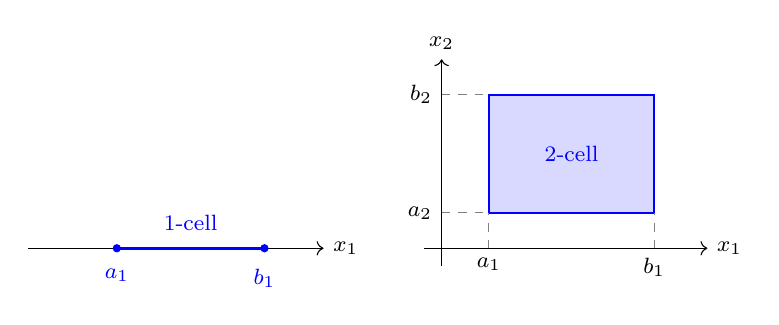
\begin{tikzpicture}[scale=0.75]
    % --- 1-cell (interval) ---
    \begin{scope}[yshift=-0.8cm]
      \draw[->] (-0.5,0) -- (4.5,0) node[right]{\footnotesize $x_1$};
      \draw[very thick, blue] (1,0) -- (3.5,0);
      \fill[blue] (1,0) circle (2pt) node[below=4pt]{\footnotesize $a_1$};
      \fill[blue] (3.5,0) circle (2pt) node[below=4pt]{\footnotesize $b_1$};
      \node[blue, above=3pt] at (2.25,0) {\footnotesize 1-cell};
    \end{scope}

    % --- 2-cell (rectangle) ---
    \begin{scope}[xshift=6.5cm, yshift=-0.8cm]
      \draw[->] (-0.3,0) -- (4.5,0) node[right]{\footnotesize $x_1$};
      \draw[->] (0,-0.3) -- (0,3.2) node[above]{\footnotesize $x_2$};

      \fill[blue!15] (0.8,0.6) rectangle (3.6,2.6);
      \draw[thick, blue] (0.8,0.6) rectangle (3.6,2.6);

      % Axis ticks
      \draw[gray, dashed] (0.8,0) -- (0.8,0.6);
      \draw[gray, dashed] (3.6,0) -- (3.6,0.6);
      \draw[gray, dashed] (0,0.6) -- (0.8,0.6);
      \draw[gray, dashed] (0,2.6) -- (0.8,2.6);
      \node[below, font=\footnotesize] at (0.8,0) {$a_1$};
      \node[below, font=\footnotesize] at (3.6,0) {$b_1$};
      \node[left, font=\footnotesize] at (0,0.6) {$a_2$};
      \node[left, font=\footnotesize] at (0,2.6) {$b_2$};

      \node[blue] at (2.2,1.6) {\footnotesize 2-cell};
    \end{scope}
  \end{tikzpicture}
  \end{center}

  \note{
    A "k"-cell is the higher-dimensional generalization of a closed interval.
    It is the set of all points in "R" to the "k" whose coordinates each lie
    within specified bounds. On the left you can see a 1-cell, which is just
    a closed interval on the real line from "a" 1 to "b" 1. On the right is a
    2-cell, which is a rectangle in the plane. Each coordinate "x" 1 ranges
    from "a" 1 to "b" 1 and "x" 2 ranges from "a" 2 to "b" 2. A 3-cell would
    be a rectangular box in three-dimensional space, and so on for higher
    dimensions. We now turn to another fundamental geometric concept.
  }
\end{frame}

% --- Build 3/4 ---
\begin{frame}{Definition 2.17: Open and Closed Balls}
  \begin{defblock}{Definition 2.17: Open and Closed Balls}
    For $\mathbf{x} \in R^k$ and $r > 0$:
    \begin{itemize}
      \item \alert{Open ball}: $B(\mathbf{x}, r) = \{\mathbf{y} \in R^k : |\mathbf{y} - \mathbf{x}| < r\}$
      \item \alert{Closed ball}: $\bar{B}(\mathbf{x}, r) = \{\mathbf{y} \in R^k : |\mathbf{y} - \mathbf{x}| \leq r\}$
    \end{itemize}
  \end{defblock}

  \begin{center}
  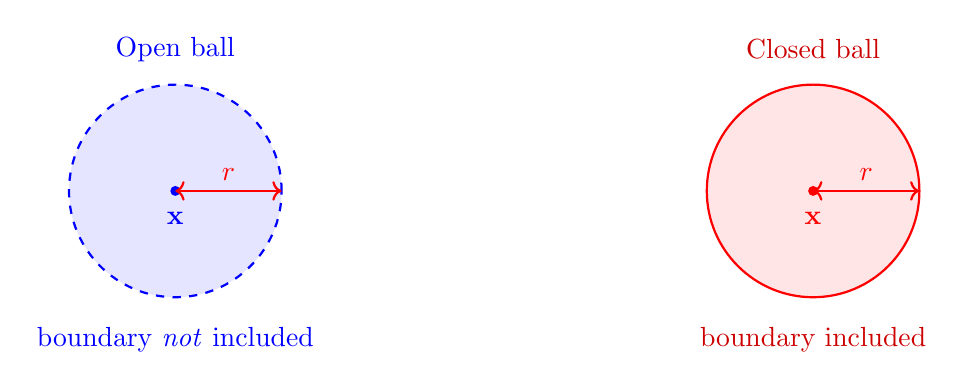
\begin{tikzpicture}[scale=0.9]
    \node[blue] at (0, 2.0) {Open ball};
    \fill[blue!10] (0,0) circle (1.5);
    \draw[thick, blue, dashed] (0,0) circle (1.5);
    \fill[blue] (0,0) circle (2pt) node[below=4pt]{$\mathbf{x}$};
    \draw[thick, red, <->] (0,0) -- (1.5,0) node[midway, above]{$r$};
    \node[blue] at (0, -2.1) {boundary \emph{not} included};

    \begin{scope}[xshift=9cm]
      \node[red!80!black] at (0, 2.0) {Closed ball};
      \fill[red!10] (0,0) circle (1.5);
      \draw[thick, red] (0,0) circle (1.5);
      \fill[red] (0,0) circle (2pt) node[below=4pt]{$\mathbf{x}$};
      \draw[thick, red, <->] (0,0) -- (1.5,0) node[midway, above]{$r$};
      \node[red!80!black] at (0, -2.1) {boundary included};
    \end{scope}
  \end{tikzpicture}
  \end{center}

  \note{
    Open and closed balls generalize segments and intervals to any dimension.
    The key distinction is whether boundary points are included. This matters
    because open balls are the building blocks of all topological concepts in
    metric spaces: neighborhoods, open sets, continuity, and convergence are
    all defined in terms of open balls. In "R" 1, an open ball is just a
    segment. In "R" 2, it is an open disk. In higher dimensions, the shape
    depends on the metric, but the concept is the same. Next we introduce an
    important geometric property.
  }
\end{frame}

% --- Build 4/5 ---
\begin{frame}{Definition 2.17: Convex Sets}
  \begin{defblock}{Definition 2.17: Convexity}
    A set $E \subset R^k$ is \alert{convex} if
    \[
      \lambda\mathbf{x} + (1 - \lambda)\mathbf{y} \in E
    \]
    whenever $\mathbf{x} \in E$, $\mathbf{y} \in E$, and $0 < \lambda < 1$.
  \end{defblock}

  \vspace{0.3em}
  \hl{\textbf{Fact:} Balls are convex. $k$-cells are convex.}

  \note{
    A set is convex if for any two points in the set, the entire line segment
    connecting them also lies in the set. Balls and "k"-cells are both convex,
    as one can verify using the triangle inequality for balls and the
    definition of "k"-cells. Let us look at a diagram to see the difference
    between convex and non-convex sets.
  }
\end{frame}

% --- Build 5/5 ---
\begin{frame}[c]{Definition 2.17: Convex vs.\ Non-Convex Sets}
  \begin{center}
  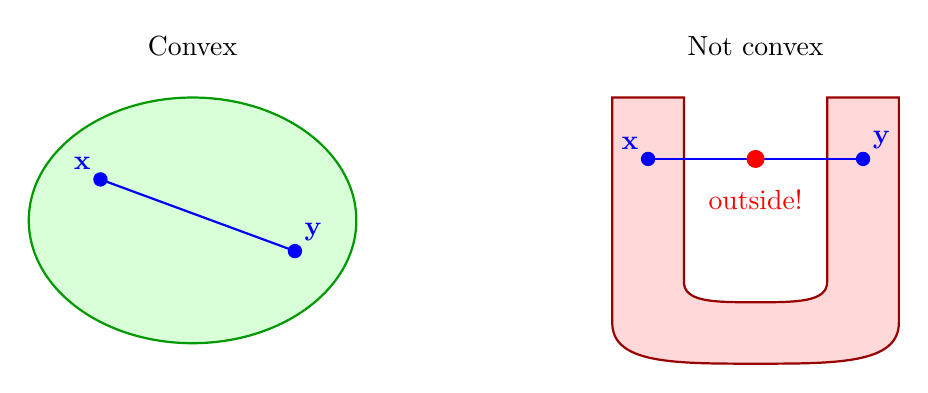
\begin{tikzpicture}[scale=1.3]
    % Convex set
    \node at (0,1.7) {Convex};
    \fill[green!15] (0,0) ellipse (1.6 and 1.2);
    \draw[thick, green!60!black] (0,0) ellipse (1.6 and 1.2);
    \fill[blue] (-0.9,0.4) circle (2pt) node[above left]{$\mathbf{x}$};
    \fill[blue] (1.0,-0.3) circle (2pt) node[above right]{$\mathbf{y}$};
    \draw[thick, blue] (-0.9,0.4) -- (1.0,-0.3);

    % Non-convex U-shaped set
    \begin{scope}[xshift=5.5cm]
      \node at (0,1.7) {Not convex};
      \fill[red!15]
        (-1.4,1.2) -- (-1.4,-1.0)
        .. controls (-1.4,-1.4) and (-0.8,-1.4) .. (0,-1.4)
        .. controls (0.8,-1.4) and (1.4,-1.4) .. (1.4,-1.0)
        -- (1.4,1.2) -- (0.7,1.2) -- (0.7,-0.6)
        .. controls (0.7,-0.8) and (0.4,-0.8) .. (0,-0.8)
        .. controls (-0.4,-0.8) and (-0.7,-0.8) .. (-0.7,-0.6)
        -- (-0.7,1.2) -- cycle;
      \draw[thick, red!60!black]
        (-1.4,1.2) -- (-1.4,-1.0)
        .. controls (-1.4,-1.4) and (-0.8,-1.4) .. (0,-1.4)
        .. controls (0.8,-1.4) and (1.4,-1.4) .. (1.4,-1.0)
        -- (1.4,1.2) -- (0.7,1.2) -- (0.7,-0.6)
        .. controls (0.7,-0.8) and (0.4,-0.8) .. (0,-0.8)
        .. controls (-0.4,-0.8) and (-0.7,-0.8) .. (-0.7,-0.6)
        -- (-0.7,1.2) -- cycle;
      \fill[blue] (-1.05,0.6) circle (2pt) node[above left]{$\mathbf{x}$};
      \fill[blue] (1.05,0.6) circle (2pt) node[above right]{$\mathbf{y}$};
      \draw[thick, blue] (-1.05,0.6) -- (1.05,0.6);
      \fill[red] (0,0.6) circle (2.5pt);
      \node[red] at (0,0.2) {outside!};
    \end{scope}
  \end{tikzpicture}
  \end{center}

  \note{
    On the left we have a convex set. Any two points "x" and "y" inside the
    set can be connected by a line segment that stays entirely within the set.
    On the right we have a non-convex set. The points "x" and "y" both belong
    to the set, but the line segment between them passes through a region
    outside the set. That single violation is enough to make the set
    non-convex.
  }
\end{frame}
}

{
\usebackgroundtemplate{%
  
\includegraphics[width=\paperwidth,height=\paperheight,keepaspectratio=false]{chapter_02_bg_02.png}%
}
% =============================================================================
\section{Topological Concepts}

% =============================================================================
% --- 2.18 Definition: Topological Vocabulary ---
% =============================================================================

% --- Build 1/5 ---
\begin{frame}{Definition 2.18: Topological Vocabulary}
  \hl{Let $X$ be a metric space. All points and sets are elements and subsets of $X$.}

  \begin{defblock}{Definition 2.18(a): Neighborhood}
    A \alert{neighborhood} of $p$ is a set $N_r(p)$ consisting of all $q$ such that
    $d(p, q) < r$, for some $r > 0$.
  \end{defblock}

  \begin{center}
  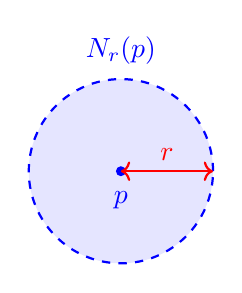
\begin{tikzpicture}[scale=0.9]
    \fill[blue!10] (0,0) circle (1.3);
    \draw[thick, blue, dashed] (0,0) circle (1.3);
    \fill[blue] (0,0) circle (2pt) node[below=4pt]{$p$};
    \draw[thick, red, <->] (0,0) -- (1.3,0) node[midway, above]{$r$};
    \node[blue] at (0,1.7) {$N_r(p)$};
  \end{tikzpicture}
  \end{center}

  \note{
    We now introduce the most important collection of definitions in this
    section. These definitions form the vocabulary of topology. A neighborhood
    of a point "p" is simply an open ball centered at "p" with some positive
    radius "r". It contains all points whose distance from "p" is strictly less
    than "r". In the real line, neighborhoods are open segments. In the plane,
    neighborhoods are open disks. Next we define when points accumulate near
    boundaries of sets.
  }
\end{frame}

% --- Build 2/5 ---
\begin{frame}{Definition 2.18: Topological Vocabulary}
  \begin{defblock}{Definition 2.18(b)--(c): Limit Points and Isolated Points}
    \begin{itemize}
      \item[(b)] $p$ is a \alert{limit point} of $E$ if \emph{every} neighborhood of $p$ contains
        a point $q \neq p$ with $q \in E$.
      \item[(c)] If $p \in E$ and $p$ is \emph{not} a limit point of $E$, then $p$ is an
        \alert{isolated point} of $E$.
    \end{itemize}
  \end{defblock}

  \begin{center}
  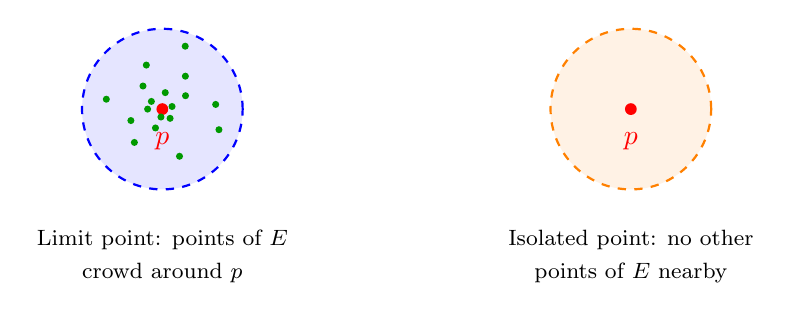
\begin{tikzpicture}[scale=0.85]
    % Limit point
    \fill[blue!10] (0,0) circle (1.2);
    \draw[thick, blue, dashed] (0,0) circle (1.2);
    \fill[red] (0,0) circle (2.5pt) node[below=5pt]{$p$};
    \foreach \a/\r in {30/0.4, 110/0.7, 200/0.5, 340/0.9, 70/1.0, 250/0.3,
      15/0.15, 145/0.2, 260/0.12, 80/0.25, 310/0.18, 180/0.22,
      55/0.6, 170/0.85, 290/0.75, 230/0.65, 5/0.8, 130/0.45}
      \fill[green!60!black] (\a:\r) circle (1.5pt);
    \node[align=center] at (0,-2.2) {\footnotesize Limit point: points of $E$\\\footnotesize crowd around $p$};

    % Isolated point
    \begin{scope}[xshift=7cm]
      \fill[orange!10] (0,0) circle (1.2);
      \draw[thick, orange, dashed] (0,0) circle (1.2);
      \fill[red] (0,0) circle (2.5pt) node[below=5pt]{$p$};
      \node[align=center] at (0,-2.2) {\footnotesize Isolated point: no other\\\footnotesize points of $E$ nearby};
    \end{scope}
  \end{tikzpicture}
  \end{center}

  \note{
    A limit point of a set "E" is a point "p" such that every neighborhood of
    "p", no matter how small, contains at least one point of "E" different
    from "p". The points of "E" crowd around "p". Note that "p" itself does
    not have to belong to "E". An isolated point is the opposite: it belongs
    to "E", but some neighborhood of it contains no other points of "E". It
    sits alone, separated from the rest of the set. Now we define properties
    based on limit points and interiors.
  }
\end{frame}

% --- Build 3/5 ---
\begin{frame}{Definition 2.18: Topological Vocabulary}
  \begin{defblock}{Definition 2.18(d)--(f): Closed, Interior, Open}
    \begin{itemize}
      \item[(d)] $E$ is \alert{closed} if every limit point of $E$ is a point of $E$.
      \item[(e)] $p$ is an \alert{interior point} of $E$ if there is a neighborhood $N$ of $p$
        with $N \subset E$.
      \item[(f)] $E$ is \alert{open} if every point of $E$ is an interior point of $E$.
    \end{itemize}
  \end{defblock}

  \begin{center}
  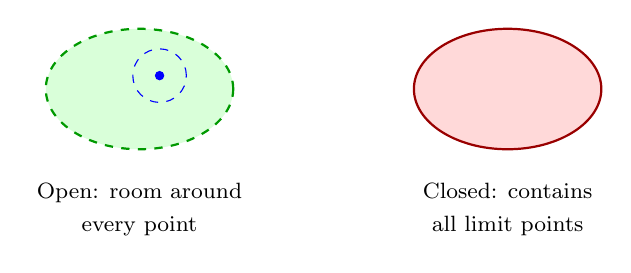
\begin{tikzpicture}[scale=0.85]
    % Open set
    \fill[green!15] (0,0) ellipse (1.4 and 0.9);
    \draw[thick, green!60!black, dashed] (0,0) ellipse (1.4 and 0.9);
    \fill[blue] (0.3,0.2) circle (2pt);
    \draw[blue, dashed] (0.3,0.2) circle (0.4);
    \node[align=center] at (0,-1.8) {\footnotesize Open: room around\\\footnotesize every point};

    % Closed set
    \begin{scope}[xshift=5.5cm]
      \fill[red!15] (0,0) ellipse (1.4 and 0.9);
      \draw[thick, red!60!black] (0,0) ellipse (1.4 and 0.9);

      \node[align=center] at (0,-1.8) {\footnotesize Closed: contains\\\footnotesize all limit points};
    \end{scope}
  \end{tikzpicture}
  \end{center}

  \note{
    A crucial subtlety here: open and closed are not opposites. A set can be
    both open and closed, like the whole space "X" or the empty set. A set
    can also be neither, like a half-open interval. Think of "closed" as
    meaning the set traps its limit points: you cannot escape by approaching
    the boundary. "Open" means every point has breathing room. These are
    independent properties that happen to be linked through complements, as
    we will see in Theorem 2.23. We now introduce the complement and a
    special type of closed set.
  }
\end{frame}

% --- Build 4/5 ---
\begin{frame}{Definition 2.18: Topological Vocabulary}
  \begin{defblock}{Definition 2.18(g)--(h): Complement and Perfect}
    \begin{itemize}
      \item[(g)] The \alert{complement} of $E$ is $E^c = \{p \in X : p \notin E\}$.
      \item[(h)] $E$ is \alert{perfect} if $E$ is closed and every point of $E$ is a limit
        point of $E$.
    \end{itemize}
  \end{defblock}

  \vspace{0.5em}
  \hl{Perfect $=$ closed $+$ no isolated points.}

  \note{
    The complement of "E" is the set of all points in "X" that do not belong
    to "E". A set is perfect if it is closed and has no isolated points. That
    means it contains all its limit points, and every point in it is a limit
    point. So a perfect set has a very uniform structure: every point is
    crowded by other points of the set, and nothing is missing from the
    boundary. A closed interval like the set of all "x" between 0 and 1 is
    a simple example of a perfect set. Finally, we define the remaining
    topological properties.
  }
\end{frame}

% --- Build 5/5 ---
\begin{frame}{Definition 2.18: Topological Vocabulary}
  \begin{defblock}{Definition 2.18(i)--(j): Bounded and Dense}
    \begin{itemize}
      \item[(i)] $E$ is \alert{bounded} if there exist $M > 0$ and $q \in X$ such that
        $d(p, q) < M$ for all $p \in E$.
      \item[(j)] $E$ is \alert{dense in $X$} if every point of $X$ is a limit point of $E$,
        or a point of $E$ (or both).
    \end{itemize}
  \end{defblock}

  \vspace{0.3em}
  \begin{hlbox}
    \textbf{Note:}
    \begin{itemize}
      \item In $R^1$ neighborhoods are segments
      \item In $R^2$ neighborhoods are open disks
    \end{itemize}
  \end{hlbox}

  \note{
    A set is bounded if it can be contained within some large ball. There is
    a single ball big enough to hold all of "E". A set is dense in "X" if it
    comes arbitrarily close to every point of "X". The rationals are dense in
    the reals, for example, because between any two real numbers there is a
    rational. This completes our topological vocabulary. These ten definitions
    are the building blocks for everything that follows in this chapter.
  }
\end{frame}

% =============================================================================
% --- 2.19 Theorem: Every neighborhood is open ---
% =============================================================================

\begin{frame}{Theorem 2.19: Every Neighborhood Is an Open Set}
  \begin{thmblock}{Theorem 2.19}
    Every neighborhood is an open set.
  \end{thmblock}

  \note{
    Our first theorem says that neighborhoods, which we defined as open
    balls, are indeed open sets in the sense of Definition 2.18. This is
    reassuring: the terminology is consistent. Let us prove this.
  }
\end{frame}

% --- Proof of 2.19 ---
\begin{frame}{Proof of Theorem 2.19}
  \begin{proofblock}{Proof}
    Let $E = N_r(p)$ and let $q \in E$. Set $h = r - d(p,q) > 0$.

    For any $s$ with $d(q, s) < h$:
    \[
      d(p, s) \leq d(p, q) + d(q, s) < (r - h) + h = r
    \]
    So $s \in E$. Thus $N_h(q) \subset E$, and $q$ is an interior point. \qed
  \end{proofblock}

  \note{
    The proof uses the triangle inequality. Take any point "q" in the
    neighborhood of "p" with radius "r". The distance from "p" to "q" is less
    than "r", so there is a positive gap "h" equal to "r" minus that distance.
    We claim the smaller neighborhood of "q" with radius "h" fits entirely
    inside the original neighborhood. For any point "s" within distance "h"
    of "q", the triangle inequality gives us that the distance from "p" to "s"
    is less than "r". Let us look at a diagram to see this visually.
  }
\end{frame}

% --- Diagram for Proof of 2.19 ---
\begin{frame}[c]{Proof of Theorem 2.19 --- Diagram}
  \begin{center}
  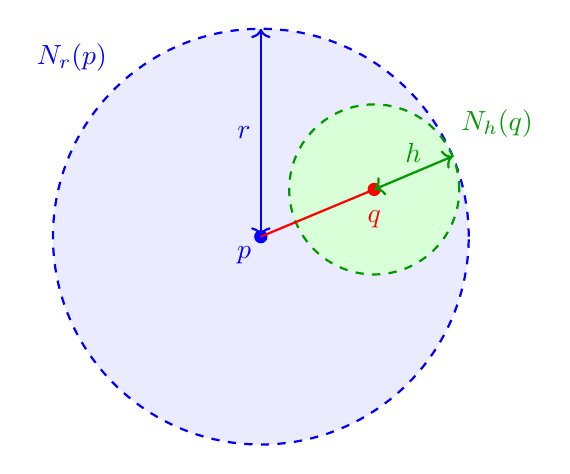
\begin{tikzpicture}[scale=1.2]
    \fill[blue!8] (0,0) circle (2.2);
    \draw[thick, blue, dashed] (0,0) circle (2.2);
    \fill[blue] (0,0) circle (2pt) node[below left]{$p$};

    \fill[green!15] (1.2,0.5) circle (0.9);
    \draw[thick, green!60!black, dashed] (1.2,0.5) circle (0.9);
    \fill[red] (1.2,0.5) circle (2pt) node[below=4pt]{$q$};

    \draw[thick, blue, <->] (0,0) -- (0,2.2) node[midway, left]{$r$};
    \draw[thick, red] (0,0) -- (1.2,0.5);
    \draw[thick, green!60!black, <->] (1.2,0.5) -- (2.03,0.85) node[midway, above]{$h$};

    \node[blue] at (-2.0, 1.9) {$N_r(p)$};
    \node[green!60!black] at (2.5, 1.2) {$N_h(q)$};
  \end{tikzpicture}
  \end{center}

  \note{
    The diagram makes the geometry clear. The key insight is how we chose the
    radius "h" of the green ball. It equals exactly the gap between "q" and
    the boundary of the blue ball. This guarantees the green ball cannot
    poke outside the blue one. This technique of choosing a radius equal to
    the remaining gap appears repeatedly in topology proofs. Whenever you
    need to show a point is interior, you compute how much room is left and
    use that as the radius of a smaller neighborhood.
  }
\end{frame}

% =============================================================================
% --- 2.20 Theorem: Limit points give infinitely many points ---
% =============================================================================

\begin{frame}{Theorem 2.20: Limit Points Yield Infinitely Many Points}
  \begin{thmblock}{Theorem 2.20}
    If $p$ is a limit point of $E$, then every neighborhood of $p$ contains
    \alert{infinitely many} points of $E$.
  \end{thmblock}

  \note{
    This theorem strengthens the definition of a limit point. The definition
    only requires that every neighborhood of "p" contains at least one point
    of "E" different from "p". But the theorem says that if even one such
    point exists in every neighborhood, then in fact infinitely many must
    exist. Let us see why.
  }
\end{frame}

% --- Proof of 2.20 ---
\begin{frame}{Proof of Theorem 2.20}
  \begin{proofblock}{Proof (by contradiction)}
    Suppose some neighborhood $N$ of $p$ contains only finitely many points
    of $E$ (other than $p$): call them $q_1, \dots, q_n$.

    \vspace{0.3em}
    Let $r = \min_{1 \leq m \leq n} d(p, q_m) > 0$.

    \vspace{0.3em}
    Then $N_r(p)$ contains \emph{no} point of $E$ other than $p$
    \;$\Longrightarrow$\; $p$ is not a limit point. \alert{Contradiction!} \qed
  \end{proofblock}

  \vspace{0.5em}
  \hl{\textbf{Corollary:}\; A finite point set has no limit points.}

  \note{
    The proof is a clever contradiction argument. If some neighborhood of
    "p" contained only finitely many points of "E" other than "p", we could
    take the minimum of the distances from "p" to each of these finitely many
    points. This minimum is positive because there are only finitely many
    points. A neighborhood of "p" with this smaller radius would then
    contain no point of "E" other than "p", contradicting the assumption
    that "p" is a limit point. The corollary follows immediately: if "E" is
    finite, no point can have infinitely many points of "E" nearby, so there
    are no limit points.
  }
\end{frame}

% =============================================================================
% --- 2.21 Examples ---
% =============================================================================

% --- Build 1/3 ---
\begin{frame}{Examples 2.21: Subsets of $R^2$}
  \begin{exblock}{Examples 2.21}
    Consider the following subsets:
    \begin{enumerate}
      \item[(a)] $\{z \in \mathbb{C} : |z| < 1\}$ --- open unit disk
      \item[(b)] $\{z \in \mathbb{C} : |z| \leq 1\}$ --- closed unit disk
      \item[(c)] A nonempty finite set
    \end{enumerate}
  \end{exblock}

  \note{
    Concrete examples are the best way to build intuition for these abstract
    definitions. As we go through these seven subsets of "R" 2, pay attention
    to how properties like open, closed, and perfect interact. You will see
    that some familiar sets have surprising properties, and that seemingly
    simple sets can behave differently depending on the ambient space. Now
    we examine more examples.
  }
\end{frame}

% --- Build 2/3 ---
% (kept on bg_02 — inside the same section)
\begin{frame}{Examples 2.21: Subsets of $R^2$}
  \begin{exblock}{Examples 2.21 (continued)}
    \begin{enumerate}
      \item[(d)] The set of all integers $\mathbb{Z}$
      \item[(e)] $\{1/n : n = 1, 2, 3, \dots\}$
      \item[(f)] $\mathbb{C}$ (all complex numbers, i.e., $R^2$)
      \item[(g)] The segment $(a, b)$
    \end{enumerate}
  \end{exblock}

  \vspace{0.3em}
  \hl{\textbf{Note on (e):} $E$ has a limit point ($z = 0$) that is \emph{not in} $E$.}

  \note{
    Set (d) is the integers. Set (e) is the sequence of reciprocals: 1, 1/2,
    1/3, and so on. This set has an interesting property: zero is a limit
    point of "E" because the reciprocals get arbitrarily close to zero, but
    zero itself is not in "E". This illustrates the distinction between having
    a limit point and containing it. Set (f) is the entire plane, and set (g)
    is an open segment on the real line. Let us now summarize the properties
    of all these sets in a table.
  }
\end{frame}

% --- Build 3/3 ---
\begin{frame}{Examples 2.21: Subsets of $R^2$}
  \begin{exblock}{Properties Table}
    \begin{center}
    \begin{tabular}{lcccc}
      & \emph{Closed} & \emph{Open} & \emph{Perfect} & \emph{Bounded} \\[3pt]
      (a) open disk & No & Yes & No & Yes \\
      (b) closed disk & Yes & No & Yes & Yes \\
      (c) finite set & Yes & No & No & Yes \\
      (d) $\mathbb{Z}$ & Yes & No & No & No \\
      (e) $\{1/n\}$ & No & No & No & Yes \\
      (f) $\mathbb{C}$ & Yes & Yes & Yes & No \\
      (g) $(a,b)$ & No & $*$ & No & Yes \\
    \end{tabular}
    \end{center}
  \end{exblock}

  \hl{$*$ Open in $R^1$ but not in $R^2$!}

  \note{
    This table summarizes the properties of each set. Notice some
    interesting points. The entire space, set (f), is both open and closed.
    That might seem contradictory, but it is perfectly consistent with the
    definitions. The segment in (g) is open as a subset of "R" 1, but not as a
    subset of "R" 2. This shows that topological properties depend on the
    ambient space, which motivates the concept of relative topology that we
    will discuss later.
  }
\end{frame}
}

{
\usebackgroundtemplate{%
  
\includegraphics[width=\paperwidth,height=\paperheight,keepaspectratio=false]{chapter_02_bg_03.png}%
}
% =============================================================================
\section{Open and Closed Sets}

% =============================================================================
% --- 2.22 Theorem: De Morgan's Law ---
% =============================================================================

\begin{frame}{Theorem 2.22: De Morgan's Law for Sets}
  \begin{thmblock}{Theorem 2.22}
    For any collection $\{E_\alpha\}$ of sets:
    \[
      \left(\bigcup_\alpha E_\alpha\right)^c = \bigcap_\alpha (E_\alpha^c)
    \]
  \end{thmblock}

  \note{
    This is De Morgan's law for sets. The complement of a union is the
    intersection of the complements. This purely set-theoretic result will be
    the key tool for transferring results about open sets to closed sets and
    vice versa throughout this chapter.
  }
\end{frame}

% --- Proof of 2.22: A ⊂ B ---
\begin{frame}{Proof of Theorem 2.22 --- $A \subset B$}
  \begin{proofblock}{Proof: $A \subset B$}
    Let $A = \left(\bigcup_\alpha E_\alpha\right)^c$ and
    $B = \bigcap_\alpha (E_\alpha^c)$.

    \vspace{0.3em}
    $x \in A$ $\Rightarrow$ $x \notin \bigcup_\alpha E_\alpha$
    $\Rightarrow$ $x \notin E_\alpha$ for all $\alpha$
    $\Rightarrow$ $x \in E_\alpha^c$ for all $\alpha$
    $\Rightarrow$ $x \in B$.
  \end{proofblock}

  \note{
    To show two sets are equal, we show each is a subset of the other. For
    the first direction, take any "x" in "A", the complement of the union.
    Then "x" is not in the union, which means "x" is not in any of the
    individual sets "E" alpha. So "x" belongs to the complement of every "E"
    alpha, which puts "x" in the intersection of all these complements,
    namely "B". This gives us "A" is a subset of "B".
  }
\end{frame}

% --- Proof of 2.22: B ⊂ A ---
\begin{frame}{Proof of Theorem 2.22 --- $B \subset A$}
  \begin{proofblock}{Proof}
    Let $A = \left(\bigcup_\alpha E_\alpha\right)^c$ and
    $B = \bigcap_\alpha (E_\alpha^c)$.

    \vspace{0.3em}
    $x \in A$ $\Rightarrow$ $x \notin \bigcup_\alpha E_\alpha$
    $\Rightarrow$ $x \notin E_\alpha$ for all $\alpha$
    $\Rightarrow$ $x \in E_\alpha^c$ for all $\alpha$
    $\Rightarrow$ $x \in B$.

    \vspace{0.3em}
    $x \in B$ $\Rightarrow$ $x \in E_\alpha^c$ for all $\alpha$
    $\Rightarrow$ $x \notin E_\alpha$ for all $\alpha$
    $\Rightarrow$ $x \notin \bigcup_\alpha E_\alpha$
    $\Rightarrow$ $x \in A$.

    \vspace{0.3em}
    Hence $A = B$. \qed
  \end{proofblock}

  \note{
    For the reverse direction, take any "x" in "B", the intersection of the
    complements. Then "x" is in the complement of every "E" alpha, meaning
    "x" is not in any "E" alpha. So "x" is not in the union, which means "x"
    belongs to the complement of the union, namely "A". Since we have shown
    both "A" subset "B" and "B" subset "A", the two sets are equal, and the
    proof is complete.
  }
\end{frame}

% =============================================================================
% --- 2.23 Theorem: Open iff complement is closed ---
% =============================================================================

\begin{frame}{Theorem 2.23: Open Sets and Closed Complements}
  \begin{thmblock}{Theorem 2.23}
    A set $E$ is open if and only if its complement $E^c$ is closed.
  \end{thmblock}

  \vspace{0.5em}
  \hl{\textbf{Corollary:}\; A set $F$ is closed if and only if $F^c$ is open.}

  \note{
    This theorem reveals the fundamental duality between open and closed sets.
    A set is open precisely when its complement is closed, and vice versa.
    This means we can always translate a statement about open sets into one
    about closed sets by taking complements. The corollary is immediate by
    applying the theorem to the complement. Let us prove the forward direction.
  }
\end{frame}

% --- Proof of 2.23: Forward direction ---

% --- Build 1/3 ---
\begin{frame}{Proof of Theorem 2.23 --- Forward Direction}
  \begin{proofblock}{$E^c$ closed $\Longrightarrow$ $E$ open}
    Suppose $E^c$ is closed. Pick $x \in E$.

    \vspace{0.3em}
    Then $x \notin E^c$ and $x$ is not a limit point of $E^c$.
  \end{proofblock}

  \note{
    The proof strategy is elegant: we translate "openness" of "E" into a
    statement about the complement being closed. Take any "x" in "E". Since
    "x" is not in the complement, and the complement is closed, meaning it
    already contains all its limit points, "x" cannot be a limit point of
    the complement either. This is where closedness does the heavy lifting.
    We extract the key consequence.
  }
\end{frame}

% --- Build 2/3 ---
\begin{frame}{Proof of Theorem 2.23 --- Forward Direction}
  \begin{proofblock}{$E^c$ closed $\Longrightarrow$ $E$ open}
    Suppose $E^c$ is closed. Pick $x \in E$.

    \vspace{0.3em}
    Then $x \notin E^c$ and $x$ is not a limit point of $E^c$.

    \vspace{0.3em}
    So there exists a neighborhood $N$ of $x$ with $E^c \cap N = \emptyset$.

    \vspace{0.3em}
    This means $N \subset E$, so $x$ is an interior point.
  \end{proofblock}

  \note{
    Here is the crucial logical step. Not being a limit point of the
    complement means there is some neighborhood that avoids the complement
    entirely. And a neighborhood that avoids the complement must lie entirely
    inside "E". This is the bridge between limit points and interior points,
    two concepts that at first seem unrelated.
  }
\end{frame}

% --- Build 3/3 ---
\begin{frame}{Proof of Theorem 2.23 --- Forward Direction}
  \begin{proofblock}{$E^c$ closed $\Longrightarrow$ $E$ open}
    Suppose $E^c$ is closed. Pick $x \in E$.

    \vspace{0.3em}
    Then $x \notin E^c$ and $x$ is not a limit point of $E^c$.

    \vspace{0.3em}
    So there exists a neighborhood $N$ of $x$ with $E^c \cap N = \emptyset$.

    \vspace{0.3em}
    This means $N \subset E$, so $x$ is an interior point.

    \vspace{0.3em}
    Since $x$ was arbitrary, $E$ is open. \qed
  \end{proofblock}

  \note{
    Since "x" was arbitrary, every point of "E" is interior, so "E" is open.
    Notice how the proof never directly computed neighborhoods or distances.
    Instead it worked purely through logical relationships between limit
    points, complements, and interior points. This style of proof is typical
    in topology. Now let us prove the reverse direction.
  }
\end{frame}

% --- Proof of 2.23: Reverse direction ---

% --- Build 1/2 ---
\begin{frame}{Proof of Theorem 2.23 --- Reverse Direction}
  \begin{proofblock}{$E$ open $\Longrightarrow$ $E^c$ closed}
    Suppose $E$ is open. Let $x$ be a limit point of $E^c$.

    \vspace{0.3em}
    Every neighborhood of $x$ contains a point of $E^c$.

    \vspace{0.3em}
    So $x$ is \emph{not} an interior point of $E$.
  \end{proofblock}

  \note{
    For the reverse direction, suppose "E" is open and "x" is a limit point
    of the complement. Then every neighborhood of "x" contains a point of the
    complement, which means no neighborhood of "x" is entirely contained in
    "E". So "x" is not an interior point of "E". We now conclude the proof.
  }
\end{frame}

% --- Build 2/2 ---
\begin{frame}{Proof of Theorem 2.23 --- Reverse Direction}
  \begin{proofblock}{$E$ open $\Longrightarrow$ $E^c$ closed}
    Suppose $E$ is open. Let $x$ be a limit point of $E^c$.

    \vspace{0.3em}
    Every neighborhood of $x$ contains a point of $E^c$.

    \vspace{0.3em}
    So $x$ is \emph{not} an interior point of $E$.

    \vspace{0.3em}
    Since $E$ is open, $x \notin E$. Hence $x \in E^c$.

    \vspace{0.3em}
    All limit points of $E^c$ lie in $E^c$, so $E^c$ is closed. \qed
  \end{proofblock}

  \note{
    But "E" is open, meaning every point of "E" is interior. Since "x" is not
    interior, "x" cannot be in "E", so "x" must be in the complement. We have
    shown that every limit point of the complement lies in the complement,
    which means the complement is closed. This completes the proof of
    Theorem 2.23.
  }
\end{frame}

% =============================================================================
% --- 2.24 Theorem: Union/Intersection properties ---
% =============================================================================

% --- Build 1/4 ---
\begin{frame}{Theorem 2.24: Unions and Intersections}
  \begin{thmblock}{Theorem 2.24}
    \begin{enumerate}
      \item[(a)] For any collection $\{G_\alpha\}$ of open sets,
        $\bigcup_\alpha G_\alpha$ is open.
    \end{enumerate}
  \end{thmblock}

  \note{
    Theorem 2.24 tells us how open and closed sets behave under unions and
    intersections. Part (a) says that any union of open sets is open, no matter
    how many sets are in the collection. This is because if a point belongs to
    the union, it belongs to at least one of the open sets, and so it has a
    neighborhood inside that set, hence inside the union.
  }
\end{frame}

% --- Build 2/4 ---
\begin{frame}{Theorem 2.24: Unions and Intersections}
  \begin{thmblock}{Theorem 2.24}
    \begin{enumerate}
      \item[(a)] For any collection $\{G_\alpha\}$ of open sets,
        $\bigcup_\alpha G_\alpha$ is open.
      \item[(b)] For any collection $\{F_\alpha\}$ of closed sets,
        $\bigcap_\alpha F_\alpha$ is closed.
    \end{enumerate}
  \end{thmblock}

  \note{
    Part (b) is the dual statement: any intersection of closed sets is closed.
    This follows from part (a) by taking complements and applying De Morgan's
    law. The complement of the intersection of closed sets is the union of
    their complements, which are open, and that union is open by part (a). So
    the intersection is closed.
  }
\end{frame}

% --- Build 3/4 ---
\begin{frame}{Theorem 2.24: Unions and Intersections}
  \begin{thmblock}{Theorem 2.24}
    \begin{enumerate}
      \item[(a)] For any collection $\{G_\alpha\}$ of open sets,
        $\bigcup_\alpha G_\alpha$ is open.
      \item[(b)] For any collection $\{F_\alpha\}$ of closed sets,
        $\bigcap_\alpha F_\alpha$ is closed.
      \item[(c)] For any \alert{finite} collection $G_1, \dots, G_n$ of open sets,
        $\bigcap_{i=1}^n G_i$ is open.
    \end{enumerate}
  \end{thmblock}

  \note{
    Part (c) requires finiteness. A finite intersection of open sets is open.
    The proof takes the minimum of the radii of the neighborhoods at a given
    point, one for each open set. Because there are only finitely many, the
    minimum is still positive. This gives a neighborhood that fits inside all
    of the sets simultaneously. Part (d) completes the pattern.
  }
\end{frame}

% --- Build 4/4 ---
\begin{frame}{Theorem 2.24: Unions and Intersections}
  \begin{thmblock}{Theorem 2.24}
    \begin{enumerate}
      \item[(a)] For any collection $\{G_\alpha\}$ of open sets,
        $\bigcup_\alpha G_\alpha$ is open.
      \item[(b)] For any collection $\{F_\alpha\}$ of closed sets,
        $\bigcap_\alpha F_\alpha$ is closed.
      \item[(c)] For any \alert{finite} collection $G_1, \dots, G_n$ of open sets,
        $\bigcap_{i=1}^n G_i$ is open.
      \item[(d)] For any \alert{finite} collection $F_1, \dots, F_n$ of closed sets,
        $\bigcup_{i=1}^n F_i$ is closed.
    \end{enumerate}
  \end{thmblock}

  \note{
    Part (d) is the dual of part (c): a finite union of closed sets is closed.
    Again this follows from (c) by complementation. Notice the pattern: unions
    preserve openness, intersections preserve closedness, and for the reverse
    operations we need finiteness. Let us now see why finiteness is essential.
  }
\end{frame}

% --- Proof of 2.24(a) ---

% --- Build 1/2 ---
\begin{frame}{Proof of Theorem 2.24(a)}
  \begin{proofblock}{Proof of (a): Arbitrary union of open sets is open}
    Let $G = \bigcup_\alpha G_\alpha$.

    \vspace{0.3em}
    If $x \in G$, then $x \in G_\alpha$ for some $\alpha$.

    \vspace{0.3em}
    Since $G_\alpha$ is open, $x$ is an interior point of $G_\alpha$.
  \end{proofblock}

  \note{
    The proof of part (a) is beautifully simple. The key observation is that
    to show a point is interior to the union, we only need it to be interior
    to one member of the union. We do not need a neighborhood that fits
    inside all the sets at once, just one of them. That is why no finiteness
    assumption is needed here. We complete the argument.
  }
\end{frame}

% --- Build 2/2 ---
\begin{frame}{Proof of Theorem 2.24(a)}
  \begin{proofblock}{Proof of (a): Arbitrary union of open sets is open}
    Let $G = \bigcup_\alpha G_\alpha$.

    \vspace{0.3em}
    If $x \in G$, then $x \in G_\alpha$ for some $\alpha$.

    \vspace{0.3em}
    Since $G_\alpha$ is open, $x$ is an interior point of $G_\alpha$.

    \vspace{0.3em}
    So there is a neighborhood $N \subset G_\alpha \subset G$.

    \vspace{0.3em}
    Hence $x$ is an interior point of $G$, and $G$ is open. \qed
  \end{proofblock}

  \note{
    Since "G" alpha is a subset of the union "G", the neighborhood that fits
    inside "G" alpha automatically fits inside "G". Compare this with the
    intersection case, where we need to fit inside every set simultaneously.
    That difference is exactly why intersections require finiteness. Let us
    see that proof next.
  }
\end{frame}

% --- Proof of 2.24(c) ---

% --- Build 1/3 ---
\begin{frame}{Proof of Theorem 2.24(c)}
  \begin{proofblock}{Proof of (c): Finite intersection of open sets is open}
    Let $H = \bigcap_{i=1}^n G_i$. For $x \in H$:

    \vspace{0.3em}
    Each $G_i$ is open, so there exist neighborhoods $N_i$ of $x$ with radius
    $r_i$ such that $N_i \subset G_i$.
  \end{proofblock}

  \note{
    For the finite intersection, take any point "x" in the intersection "H".
    Since "x" belongs to each of the "n" open sets, for each "G" "i" there
    exists a neighborhood of "x" with some radius "r" "i" that fits inside
    "G" "i". Now we use the finiteness assumption.
  }
\end{frame}

% --- Build 2/3 ---
\begin{frame}{Proof of Theorem 2.24(c)}
  \begin{proofblock}{Proof of (c): Finite intersection of open sets is open}
    Let $H = \bigcap_{i=1}^n G_i$. For $x \in H$:

    \vspace{0.3em}
    Each $G_i$ is open, so there exist neighborhoods $N_i$ of $x$ with radius
    $r_i$ such that $N_i \subset G_i$.

    \vspace{0.3em}
    Set $r = \min(r_1, \dots, r_n) > 0$ \quad(finite minimum of positive numbers).
  \end{proofblock}

  \note{
    Now take the smallest of these "n" radii. Because there are only finitely
    many, and each is positive, the minimum "r" is still positive. This is
    exactly where finiteness is needed: an infinite minimum of positive
    numbers could be zero. We conclude by showing the intersection is open.
  }
\end{frame}

% --- Build 3/3 ---
\begin{frame}{Proof of Theorem 2.24(c)}
  \begin{proofblock}{Proof of (c): Finite intersection of open sets is open}
    Let $H = \bigcap_{i=1}^n G_i$. For $x \in H$:

    \vspace{0.3em}
    Each $G_i$ is open, so there exist neighborhoods $N_i$ of $x$ with radius
    $r_i$ such that $N_i \subset G_i$.

    \vspace{0.3em}
    Set $r = \min(r_1, \dots, r_n) > 0$ \quad(finite minimum of positive numbers).

    \vspace{0.3em}
    Then $N_r(x) \subset G_i$ for all $i$, so $N_r(x) \subset H$. \qed
  \end{proofblock}

  \note{
    The neighborhood of "x" with this minimum radius fits inside every one of
    the "n" sets, hence inside their intersection "H". So "x" is an interior
    point of "H", and since "x" was arbitrary, "H" is open. Parts (b) and (d)
    follow from (a) and (c) by taking complements and applying De Morgan's law.
  }
\end{frame}

% =============================================================================
% --- 2.25 Examples: Finiteness is essential ---
% =============================================================================

\begin{frame}{Examples 2.25: Why Finiteness Matters}
  \begin{exblock}{Example 2.25}
    Let $G_n = \left(-\dfrac{1}{n},\, \dfrac{1}{n}\right)$ for $n = 1, 2, 3, \dots$

    \vspace{0.3em}
    Each $G_n$ is open. But:
    \[
      \bigcap_{n=1}^{\infty} G_n = \{0\}
    \]
    which is \alert{not open}.
  \end{exblock}

  \begin{center}
  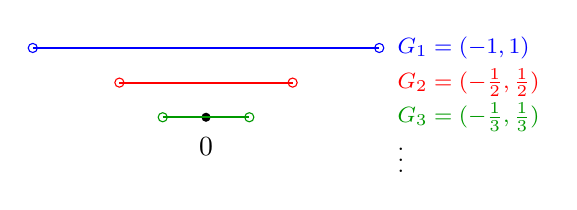
\begin{tikzpicture}[scale=1.1]
    \fill (0,0) circle (1.5pt) node[below=4pt]{$0$};

    \draw[thick, blue] (-2,0.8) -- (2,0.8);
    \draw[blue] (-2,0.8) circle (1.5pt); \draw[blue] (2,0.8) circle (1.5pt);
    \node[blue, right] at (2.1,0.8) {\footnotesize $G_1 = (-1,1)$};

    \draw[thick, red] (-1,0.4) -- (1,0.4);
    \draw[red] (-1,0.4) circle (1.5pt); \draw[red] (1,0.4) circle (1.5pt);
    \node[red, right] at (2.1,0.4) {\footnotesize $G_2 = (-\frac{1}{2},\frac{1}{2})$};

    \draw[thick, green!60!black] (-0.5,0.0) -- (0.5,0.0);
    \draw[green!60!black] (-0.5,0.0) circle (1.5pt);
    \draw[green!60!black] (0.5,0.0) circle (1.5pt);
    \node[green!60!black, right] at (2.1,0.0) {\footnotesize $G_3 = (-\frac{1}{3},\frac{1}{3})$};

    \node[right] at (2.1,-0.4) {\footnotesize $\vdots$};
  \end{tikzpicture}
  \end{center}

  \note{
    This example shows why finiteness cannot be dropped from parts (c) and
    (d) of Theorem 2.24. Each interval from minus 1 over "n" to 1 over "n"
    is open. But as "n" grows, these intervals shrink toward zero. Their
    intersection is just the single point zero, which is not open. So an
    infinite intersection of open sets need not be open. Similarly, an
    infinite union of closed sets need not be closed. Now we turn to the
    closure of sets.
  }
\end{frame}
}

{
\usebackgroundtemplate{%
  
\includegraphics[width=\paperwidth,height=\paperheight,keepaspectratio=false]{chapter_02_bg_04.png}%
}
% =============================================================================
\section{Closure and Relative Topology}

% =============================================================================
% --- 2.26 Definition: Closure ---
% =============================================================================

\begin{frame}{Definition 2.26: Closure of a Set}
  \begin{defblock}{Definition 2.26}
    If $E \subset X$ and $E'$ denotes the set of all limit points of $E$ in $X$, then
    the \alert{closure} of $E$ is:
    \[
      \bar{E} = E \cup E'
    \]
  \end{defblock}

  \begin{center}
  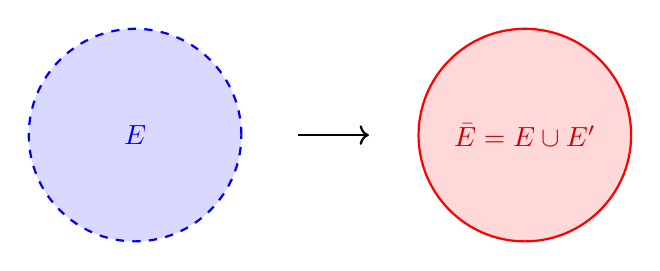
\begin{tikzpicture}[scale=0.9]
    % E (open disk)
    \fill[blue!15] (0,0) circle (1.5);
    \draw[thick, blue, dashed] (0,0) circle (1.5);
    \node[blue] at (0,0) {$E$};

    \draw[thick, ->] (2.3,0) -- (3.3,0);

    % E-bar (closed disk)
    \begin{scope}[xshift=5.5cm]
      \fill[red!15] (0,0) circle (1.5);
      \draw[thick, red] (0,0) circle (1.5);
      \node[red!80!black] at (0,0) {$\bar{E} = E \cup E'$};
    \end{scope}
  \end{tikzpicture}
  \end{center}

  \note{
    The closure of a set "E" is formed by taking "E" and adding all its limit
    points. The notation is "E" bar. Think of it as plugging all the holes in
    the boundary of "E". For instance, if "E" is an open disk, its closure is
    the closed disk: we add all the boundary points, which are the limit
    points not already in "E". The closure is the smallest closed set
    containing "E", as we will see next.
  }
\end{frame}

% =============================================================================
% --- 2.27 Theorem: Properties of Closure ---
% =============================================================================

% --- Build 1/3 ---
\begin{frame}{Theorem 2.27: Properties of Closure}
  \begin{thmblock}{Theorem 2.27}
    If $X$ is a metric space and $E \subset X$, then:
    \begin{enumerate}
      \item[(a)] $\bar{E}$ is closed.
    \end{enumerate}
  \end{thmblock}

  \note{
    Theorem 2.27 establishes the three key properties of closure. Part (a)
    says the closure is always a closed set. This is what we would hope: after
    adding all limit points, there should be no more limit points missing.
    Part (b) characterizes when closure is unnecessary.
  }
\end{frame}

% --- Build 2/3 ---
\begin{frame}{Theorem 2.27: Properties of Closure}
  \begin{thmblock}{Theorem 2.27}
    If $X$ is a metric space and $E \subset X$, then:
    \begin{enumerate}
      \item[(a)] $\bar{E}$ is closed.
      \item[(b)] $E = \bar{E}$ if and only if $E$ is closed.
    \end{enumerate}
  \end{thmblock}

  \note{
    Part (b) says that a set equals its own closure precisely when it is
    already closed. This makes perfect sense: a closed set already contains
    all its limit points, so adding them changes nothing. Conversely, if
    adding limit points does not change the set, then it must have contained
    them all along. Part (c) gives us a minimality property.
  }
\end{frame}

% --- Build 3/3 ---
\begin{frame}{Theorem 2.27: Properties of Closure}
  \begin{thmblock}{Theorem 2.27}
    If $X$ is a metric space and $E \subset X$, then:
    \begin{enumerate}
      \item[(a)] $\bar{E}$ is closed.
      \item[(b)] $E = \bar{E}$ if and only if $E$ is closed.
      \item[(c)] $\bar{E} \subset F$ for every closed set $F \subset X$ with $E \subset F$.
    \end{enumerate}
  \end{thmblock}

  \vspace{0.3em}
  \hl{By (a) and (c): $\bar{E}$ is the \alert{smallest} closed set containing $E$.}

  \note{
    Part (c) says the closure is contained in every closed set that contains
    "E". Combined with part (a), this means the closure is the smallest
    closed set containing "E". It is the most efficient way to close up "E".
    Now let us look at the proofs.
  }
\end{frame}

% --- Proof of 2.27 ---
% --- Build 1/3 ---
\begin{frame}{Proof of Theorem 2.27}
  \begin{proofblock}{Proof of (a): $\bar{E}$ is closed}
    If $p \notin \bar{E}$, then $p \notin E$ and $p \notin E'$.

    \vspace{0.3em}
    So $p$ has a neighborhood $N$ that does not intersect $E$.

    \vspace{0.3em}
    Hence the complement of $\bar{E}$ is open, so $\bar{E}$ is closed. \qed
  \end{proofblock}

  \note{
    For part (a), take a point "p" not in the closure. Then "p" is neither in
    "E" nor a limit point of "E". Since "p" is not a limit point, some
    neighborhood of "p" avoids "E" entirely. But then it also avoids the
    closure. This means the complement of the closure is open, so the closure
    is closed by Theorem 2.23. Part (b) is next.
  }
\end{frame}

% --- Build 2/3 ---
\begin{frame}{Proof of Theorem 2.27}
  \begin{proofblock}{Proof of (b): $E = \bar{E}$ iff $E$ is closed}
    ($\Rightarrow$) If $E = \bar{E}$, then $E$ is closed by (a).

    \vspace{0.3em}
    ($\Leftarrow$) If $E$ is closed, then $E' \subset E$, so $\bar{E} = E \cup E' = E$. \qed
  \end{proofblock}

  \note{
    Part (b) gives a useful test for closedness: just check whether the set
    equals its closure. If adding limit points changes nothing, the set was
    already closed. This is often the most practical way to verify a set is
    closed in proofs. Part (c) establishes a minimality property.
  }
\end{frame}

% --- Build 3/3 ---
\begin{frame}{Proof of Theorem 2.27}
  \begin{proofblock}{Proof of (c): $\bar{E} \subset F$ for closed $F \supset E$}
    If $F$ is closed and $F \supset E$:

    \vspace{0.3em}
    $E \subset F$ $\Rightarrow$ $E' \subset F'$
    \quad and \quad
    $F$ closed $\Rightarrow$ $F' \subset F$

    \vspace{0.3em}
    So $E' \subset F' \subset F$, hence $F \supset E \cup E' = \bar{E}$. \qed
  \end{proofblock}

  \note{
    For part (c), if "F" is closed and contains "E", we use two facts. First,
    since "E" is a subset of "F", every limit point of "E" is also a limit
    point of "F", so "E" prime is a subset of "F" prime. Second, since "F" is
    closed, "F" contains all its own limit points, so "F" prime is a subset
    of "F". Combining these, "E" prime is a subset of "F". So "F" contains
    both "E" and the limit points of "E", which means "F" contains the
    closure of "E". This completes all three parts of the theorem.
  }
\end{frame}

% =============================================================================
% --- 2.28 Theorem: Supremum in Closure ---
% =============================================================================

\begin{frame}{Theorem 2.28: Supremum Belongs to the Closure}
  \begin{thmblock}{Theorem 2.28}
    Let $E$ be a nonempty set of real numbers bounded above, and let
    $y = \sup E$. Then $y \in \bar{E}$.

    Hence $y \in E$ if $E$ is closed.
  \end{thmblock}

  \note{
    This theorem connects the supremum from Chapter 1 with the closure from
    topology. It says the supremum of a bounded-above set of reals always
    belongs to the closure of that set. If the set is closed, the supremum is
    actually in the set. This is a useful and intuitive result: the least
    upper bound is either in the set or is a limit point of the set. Let us
    prove this.
  }
\end{frame}

% --- Proof of 2.28 ---

% --- Build 1/3 ---
\begin{frame}{Proof of Theorem 2.28}
  \begin{proofblock}{Proof}
    If $y \in E$, then $y \in \bar{E}$.

    \vspace{0.3em}
    Suppose $y \notin E$. For every $h > 0$, there exists $x \in E$ with
    \[
      y - h < x < y
    \]
  \end{proofblock}

  \note{
    If the supremum "y" is already in "E", then it is certainly in the
    closure, and we are done. The interesting case is when "y" is not in "E".
    We claim that for every positive "h", there must be a point "x" in "E"
    strictly between "y" minus "h" and "y". Why is this true? We explain
    the key observation.
  }
\end{frame}

% --- Build 2/3 ---
\begin{frame}{Proof of Theorem 2.28}
  \begin{proofblock}{Proof}
    If $y \in E$, then $y \in \bar{E}$.

    \vspace{0.3em}
    Suppose $y \notin E$. For every $h > 0$, there exists $x \in E$ with
    \[
      y - h < x < y
    \]
    (otherwise $y - h$ would be an upper bound of $E$, contradicting $y = \sup E$).
  \end{proofblock}

  \note{
    If no such "x" existed, then every element of "E" would be at most "y"
    minus "h", making "y" minus "h" an upper bound of "E". But "y" is the
    least upper bound, so no smaller number can be an upper bound. This is a
    contradiction, so such an "x" must exist. We now conclude.
  }
\end{frame}

% --- Build 3/3 ---
\begin{frame}{Proof of Theorem 2.28}
  \begin{proofblock}{Proof}
    If $y \in E$, then $y \in \bar{E}$.

    \vspace{0.3em}
    Suppose $y \notin E$. For every $h > 0$, there exists $x \in E$ with
    \[
      y - h < x < y
    \]
    (otherwise $y - h$ would be an upper bound of $E$, contradicting $y = \sup E$).

    \vspace{0.3em}
    So every neighborhood of $y$ contains a point of $E$ $\Rightarrow$ $y \in E'$
    $\Rightarrow$ $y \in \bar{E}$. \qed
  \end{proofblock}

  \begin{center}
  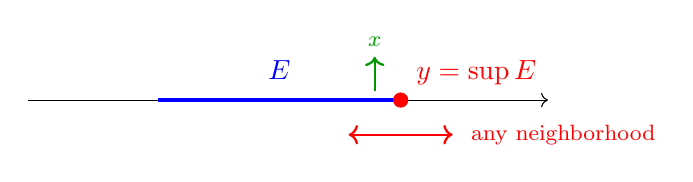
\begin{tikzpicture}[scale=1.1]
    \draw[->] (-0.5,0) -- (5.5,0);
    \draw[very thick, blue] (1,0) -- (3.8,0);
    \node[blue, above=4pt] at (2.4,0) {$E$};
    \fill[red] (3.8,0) circle (2.5pt) node[above right=3pt]{$y = \sup E$};
    \draw[thick, red, <->] (3.2,-0.4) -- (4.4,-0.4);
    \node[red, right] at (4.5,-0.4) {\footnotesize any neighborhood};
    \draw[thick, green!60!black, ->] (3.5,0.1) -- (3.5,0.5) node[above]{\footnotesize $x$};
  \end{tikzpicture}
  \end{center}

  \note{
    Since this holds for every positive "h", every neighborhood of "y"
    contains a point of "E". This makes "y" a limit point of "E", so "y"
    belongs to "E" prime and hence to the closure. As the diagram shows,
    no matter how small a neighborhood we take around "y", there is always
    a point "x" of "E" inside it.
  }
\end{frame}

% =============================================================================
% --- 2.29 Remark: Open relative to Y ---
% =============================================================================

\begin{frame}{Remark 2.29: Open Relative to a Subspace}
  \begin{remblock}{Remark 2.29}
    Suppose $E \subset Y \subset X$.

    \vspace{0.3em}
    $E$ is \alert{open relative to $Y$} if: for each $p \in E$, there exists $r > 0$
    such that
    \[
      q \in E \quad\text{whenever}\quad d(p, q) < r \;\text{ and }\; q \in Y.
    \]
  \end{remblock}

  \vspace{0.3em}
  \hl{\textbf{Recall:} $(a, b)$ is open in $R^1$ but not open in $R^2$.}

  \note{
    This remark introduces relative topology. When we ask whether a set is
    open, the answer can depend on the ambient space. A set "E" inside a
    subspace "Y" is open relative to "Y" if every point of "E" has a
    neighborhood, restricted to "Y", that stays within "E". As we saw in
    Example 2.21, the segment from "a" to "b" is open when viewed as a subset
    of the real line but not when viewed as a subset of the plane. The next
    theorem gives a clean characterization of this concept. Let us see it.
  }
\end{frame}

% =============================================================================
% --- 2.30 Theorem: Characterization of relatively open sets ---
% =============================================================================

\begin{frame}{Theorem 2.30: Characterizing Relatively Open Sets}
  \begin{thmblock}{Theorem 2.30}
    Suppose $Y \subset X$. A subset $E$ of $Y$ is open relative to $Y$ if and only if
    \[
      E = Y \cap G
    \]
    for some open subset $G$ of $X$.
  \end{thmblock}

  \note{
    This is an elegant characterization. A set is open relative to "Y" if and
    only if it is the intersection of "Y" with some set that is open in the
    full space "X". So relative openness is not a mysterious new concept; it
    always comes from restricting an open set in the ambient space to the
    subspace. Let us prove both directions. First the forward direction.
  }
\end{frame}

% --- Diagram illustrating Theorem 2.30 ---

\begin{frame}{Theorem 2.30: Illustration}
  \begin{center}
  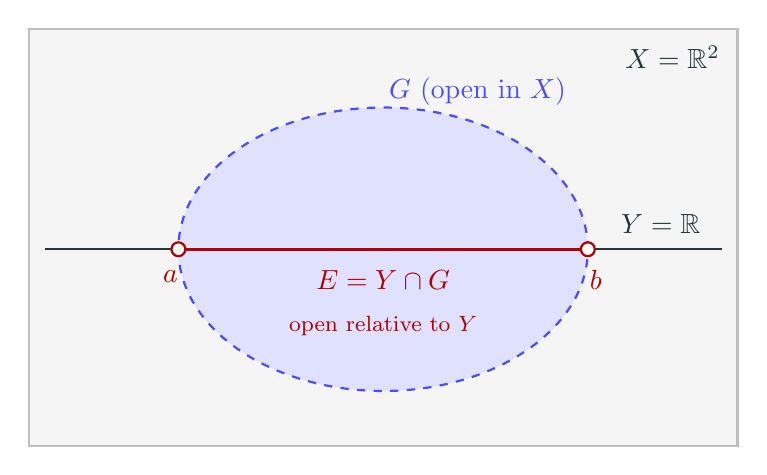
\begin{tikzpicture}[scale=1.0]
    % Ambient space X = R^2 (background rectangle)
    \fill[gray!8] (-4.5,-2.5) rectangle (4.5,2.8);
    \draw[thick, gray!50] (-4.5,-2.5) rectangle (4.5,2.8);
    \node[mDarkTeal, anchor=north east] at (4.4,2.7) {$X = \mathbb{R}^2$};

    % Open set G (ellipse/disc)
    \fill[blue!12] (0,0) ellipse (2.6cm and 1.8cm);
    \draw[thick, blue!70, dashed] (0,0) ellipse (2.6cm and 1.8cm);
    \node[blue!70, anchor=south] at (1.2,1.7) {$G$ (open in $X$)};

    % Subspace Y = real line
    \draw[thick, mDarkTeal] (-4.3,0) -- (4.3,0);
    \node[mDarkTeal, anchor=south west] at (2.9,0.08) {$Y = \mathbb{R}$};

    % E = G ∩ Y (the segment)
    \draw[very thick, red!70!black] (-2.6,0) -- (2.6,0);
    \draw[thick, red!70!black, fill=white] (-2.6,0) circle (2.5pt);
    \draw[thick, red!70!black, fill=white] (2.6,0) circle (2.5pt);
    \node[red!70!black, below=4pt] at (-2.7,0) {$a$};
    \node[red!70!black, below=4pt] at (2.7,0) {$b$};
    \node[red!70!black, below=4pt] at (0,0) {$E = Y \cap G$};

    % Brace below E
    \node[red!70!black, below=8pt] at (0,-0.45) {\footnotesize open relative to $Y$};
  \end{tikzpicture}
  \end{center}

  \note{
    Here is a concrete picture. Take "X" to be the entire plane, and "Y" to be
    the real line sitting inside it. The segment "E" from "a" to "b" is open
    relative to "Y", meaning every point in "E" has a small interval around it
    that stays inside "E". Now look at the dashed blue region "G", which is an
    open disc in the full plane. Notice that the intersection of "G" with the
    line "Y" gives exactly "E". That is the content of Theorem 2.30: every
    relatively open set arises as the trace of some open set in the ambient
    space. Conversely, any such intersection is relatively open. Let us now
    prove this formally.
  }
\end{frame}

% --- Proof of 2.30: Forward ---

% --- Build 1/2 ---
\begin{frame}{Proof of Theorem 2.30 --- Forward Direction}
  \begin{proofblock}{$E$ open relative to $Y$ $\Longrightarrow$ $E = Y \cap G$}
    For each $p \in E$, choose $r_p > 0$ so that $q \in E$ whenever
    $d(p, q) < r_p$ and $q \in Y$.

    \vspace{0.3em}
    Let $V_p = \{q \in X : d(p, q) < r_p\}$ and set $G = \bigcup_{p \in E} V_p$.

    \vspace{0.3em}
    $G$ is open in $X$ (union of neighborhoods, by Theorems 2.19 and 2.24).
  \end{proofblock}

  \note{
    For the forward direction, since "E" is open relative to "Y", for each
    point "p" in "E" we have a radius "r" sub "p" such that any point of "Y"
    within that radius belongs to "E". We form the open ball "V" sub "p" in
    the full space "X" and take the union of all these balls. This union "G"
    is open in "X" by Theorems 2.19 and 2.24. Now we need to show that "E"
    equals "G" intersected with "Y". We verify both inclusions.
  }
\end{frame}

% --- Build 2/2 ---
\begin{frame}{Proof of Theorem 2.30 --- Forward Direction}
  \begin{proofblock}{$E$ open relative to $Y$ $\Longrightarrow$ $E = Y \cap G$}
    For each $p \in E$, choose $r_p > 0$ so that $q \in E$ whenever
    $d(p, q) < r_p$ and $q \in Y$.

    \vspace{0.3em}
    Let $V_p = \{q \in X : d(p, q) < r_p\}$ and set $G = \bigcup_{p \in E} V_p$.

    \vspace{0.3em}
    $G$ is open in $X$ (union of neighborhoods, by Theorems 2.19 and 2.24).

    \vspace{0.3em}
    \textbf{Claim:} $E = G \cap Y$.
    \begin{itemize}
      \item $E \subset G \cap Y$: each $p \in E$ lies in $V_p \subset G$, and $p \in Y$.
      \item $G \cap Y \subset E$: if $q \in V_p \cap Y$, then $q \in E$ by choice of $r_p$.
    \end{itemize}
    \vspace{-0.2em}\qed
  \end{proofblock}

  \note{
    We verify both inclusions. First, every point "p" in "E" lies in its own
    ball "V" sub "p", hence in "G", and "p" is in "Y", so "E" is a subset of
    "G" intersect "Y". Conversely, any point "q" in "G" intersect "Y" belongs
    to some "V" sub "p" and to "Y", so by the choice of "r" sub "p", "q" is
    in "E". Therefore "E" equals "G" intersect "Y". Now let us prove the
    converse direction.
  }
\end{frame}

% --- Proof of 2.30: Converse ---

% --- Build 1/2 ---
\begin{frame}{Proof of Theorem 2.30 --- Converse Direction}
  \begin{proofblock}{$E = Y \cap G$ with $G$ open $\Longrightarrow$ $E$ open relative to $Y$}
    If $G$ is open in $X$ and $E = G \cap Y$:

    \vspace{0.3em}
    For every $p \in E$, since $p \in G$ and $G$ is open, there exists
    a neighborhood $V_p \subset G$.
  \end{proofblock}

  \note{
    The converse is more straightforward. If we already have "E" as the
    intersection of "Y" with an open set "G" in the full space, we just need
    to show points of "E" have relative neighborhoods inside "E". Since "G"
    is open in "X", each point of "E" has a full neighborhood inside "G".
    We restrict to "Y" to finish.
  }
\end{frame}

% --- Build 2/2 ---
\begin{frame}{Proof of Theorem 2.30 --- Converse Direction}
  \begin{proofblock}{$E = Y \cap G$ with $G$ open $\Longrightarrow$ $E$ open relative to $Y$}
    If $G$ is open in $X$ and $E = G \cap Y$:

    \vspace{0.3em}
    For every $p \in E$, since $p \in G$ and $G$ is open, there exists
    a neighborhood $V_p \subset G$.

    \vspace{0.3em}
    Then $V_p \cap Y \subset G \cap Y = E$.

    \vspace{0.3em}
    So $E$ is open relative to $Y$. \qed
  \end{proofblock}

  \note{
    Restricting to "Y" gives us that "V" sub "p" intersected with "Y" lies
    inside "G" intersected with "Y", which is "E". So the relative
    neighborhood condition is satisfied. The beauty of this theorem is that
    it reduces the relative topology on "Y" to a simple intersection
    operation. You do not need to re-derive open sets from scratch in the
    subspace; you just slice open sets from the ambient space with "Y".
  }
\end{frame}
}

{
\usebackgroundtemplate{%
  
\includegraphics[width=\paperwidth,height=\paperheight,keepaspectratio=false]{chapter_02_bg_05.png}%
}
% =============================================================================
\section{Summary}

% =============================================================================
% --- Summary ---
% =============================================================================

% --- Build 1/4 ---
\begin{frame}{Summary}
  \begin{hlbox}
    \textbf{Key takeaways from this section:}
    \begin{itemize}
      \item A \alert{metric space} is a set with a distance function satisfying
        positivity, symmetry, and the triangle inequality (Def.\ 2.15).
    \end{itemize}
  \end{hlbox}

  \note{
    Let us review the main ideas from this section. We started by defining
    metric spaces as sets equipped with a distance function satisfying three
    natural axioms. Euclidean spaces are the primary examples. Next we
    introduced fundamental topological concepts.
  }
\end{frame}

% --- Build 2/4 ---
\begin{frame}{Summary}
  \begin{hlbox}
    \textbf{Key takeaways from this section:}
    \begin{itemize}
      \item A \alert{metric space} is a set with a distance function satisfying
        positivity, symmetry, and the triangle inequality (Def.\ 2.15).
      \item The topological vocabulary --- neighborhoods, limit points, open/closed
        sets, interior, closure, bounded, dense, perfect --- provides the
        language for analysis in metric spaces (Def.\ 2.18).
    \end{itemize}
  \end{hlbox}

  \note{
    We then introduced the fundamental topological vocabulary: neighborhoods,
    limit points, isolated points, open and closed sets, interior points,
    complements, boundedness, density, and perfectness. These ten concepts
    are the foundation for everything in this chapter. Then we proved key
    properties about these sets.
  }
\end{frame}

% --- Build 3/4 ---
\begin{frame}{Summary}
  \begin{hlbox}
    \textbf{Key takeaways from this section:}
    \begin{itemize}
      \item A \alert{metric space} is a set with a distance function satisfying
        positivity, symmetry, and the triangle inequality (Def.\ 2.15).
      \item The topological vocabulary --- neighborhoods, limit points, open/closed
        sets, interior, closure, bounded, dense, perfect --- provides the
        language for analysis in metric spaces (Def.\ 2.18).
      \item Open and closed are \emph{dual}: $E$ is open iff $E^c$ is closed (Thm.\ 2.23).
        Unions of open sets are open; intersections of
        closed sets are closed. Finiteness is needed for the reverse (Thm.\ 2.24).
    \end{itemize}
  \end{hlbox}

  \note{
    We proved the fundamental duality between open and closed sets via
    complements, and established the union and intersection rules. A key
    subtlety is that finiteness is required for intersections of open sets
    and unions of closed sets. Next we discussed closure.
  }
\end{frame}

% --- Build 4/5 ---
\begin{frame}{Summary}
  \begin{hlbox}
    \textbf{Key takeaways from this section:}
    \begin{itemize}
      \item A \alert{metric space} is a set with a distance function satisfying
        positivity, symmetry, and the triangle inequality (Def.\ 2.15).
      \item The topological vocabulary --- neighborhoods, limit points, open/closed
        sets, interior, closure, bounded, dense, perfect --- provides the
        language for analysis in metric spaces (Def.\ 2.18).
      \item Open and closed are \emph{dual}: $E$ is open iff $E^c$ is closed (Thm.\ 2.23).
        Unions of open sets are open; intersections of
        closed sets are closed. Finiteness is needed for the reverse (Thm.\ 2.24).
      \item The \alert{closure} $\bar{E} = E \cup E'$ is the smallest closed set containing $E$
        (Thm.\ 2.27). Relatively open sets are: $E = Y \cap G$
        (Thm.\ 2.30).
    \end{itemize}
  \end{hlbox}

  \note{
    Finally, we defined the closure as the set together with its limit
    points, proved it is the smallest closed set containing the original set,
    and characterized relatively open sets as intersections of a subspace
    with an open set in the ambient space.
  }
\end{frame}

% --- Build 5/5 ---
\begin{frame}{Coming Up Next}
  \begin{center}
    \hl{\textbf{Coming up next:} Compact sets --- a powerful finiteness condition.}
  \end{center}

  \note{
    In the next section, we will study compact sets, which introduce a
    powerful finiteness condition that has far-reaching consequences
    throughout analysis. See you there!
  }
\end{frame}
}

\end{document}
